%----------------------------------------------------------------------------------------
%	PACKAGES AND OTHER DOCUMENT CONFIGURATIONS
%----------------------------------------------------------------------------------------

\documentclass[12pt]{article}
\usepackage[english]{babel}
\usepackage[utf8x]{inputenc}
\usepackage{amsmath}
\usepackage{graphicx}
\usepackage[colorinlistoftodos]{todonotes}
\usepackage{ragged2e}
\usepackage[none]{hyphenat}
\usepackage[hidelinks]{hyperref}
\usepackage{listings}
\usepackage[title,titletoc,toc]{appendix}
\usepackage{kantlipsum}
\usepackage{spverbatim}
\usepackage{caption3}
\usepackage{longtable}
% This is for adding extra subsections
\usepackage{titlesec}
\titleclass{\subsubsubsection}{straight}[\subsection]
\newcounter{subsubsubsection}[subsubsection]
\renewcommand\thesubsubsubsection{\thesubsubsection.\arabic{subsubsubsection}}
\renewcommand\theparagraph{\thesubsubsubsection.\arabic{paragraph}}
\renewcommand\thesubparagraph{\theparagraph.\arabic{subparagraph}}

\usepackage{chngcntr}
\counterwithin{figure}{section}

\titleformat{\subsubsubsection}
  {\normalfont\normalsize\bfseries}{\thesubsubsubsection}{1em}{}
\titlespacing*{\subsubsubsection}
{0pt}{3.25ex plus 1ex minus .2ex}{1.5ex plus .2ex}

\makeatletter
\renewcommand\paragraph{\@startsection{paragraph}{5}{\z@}%
  {3.25ex \@plus1ex \@minus.2ex}%
  {-1em}%
  {\normalfont\normalsize\bfseries}}
\renewcommand\subparagraph{\@startsection{subparagraph}{6}{\parindent}
  {3.25ex \@plus1ex \@minus .2ex}%
  {-1em}%
  {\normalfont\normalsize\bfseries}}
\def\toclevel@subsubsubsection{4}
\def\toclevel@paragraph{5}
\def\toclevel@paragraph{6}
\def\l@subsubsubsection{\@dottedtocline{4}{7em}{4em}}
\def\l@paragraph{\@dottedtocline{5}{10em}{5em}}
\def\l@subparagraph{\@dottedtocline{6}{14em}{6em}}
\@addtoreset{subsubsubsection}{section}
\@addtoreset{subsubsubsection}{subsection}
\@addtoreset{paragraph}{subsubsubsection}
\makeatother
\setcounter{secnumdepth}{4}
\setcounter{tocdepth}{5}
%-----------------------------------------------%

\usepackage{array}
\newcolumntype{L}[1]{>{\raggedright\let\newline\\\arraybackslash\hspace{0pt}}m{#1}}
\newcolumntype{C}[1]{>{\centering\let\newline\\\arraybackslash\hspace{0pt}}m{#1}}
\newcolumntype{R}[1]{>{\raggedleft\let\newline\\\arraybackslash\hspace{0pt}}m{#1}}

\begin{document}

\begin{titlepage}

\newcommand{\HRule}{\rule{\linewidth}{0.5mm}} 
\center

%----------------------------------------------------------------------------------------
%	LOGO SECTION
%----------------------------------------------------------------------------------------


\includegraphics{images/uva.jpeg}\\[0.5cm]% Include a department/university logo - this will require the graphicx package
 
%----------------------------------------------------------------------------------------

%----------------------------------------------------------------------------------------
%	HEADING SECTIONS
%----------------------------------------------------------------------------------------
\textsc{\Large System and Network Engineering, MSc}\\[0.5cm] 
\textsc { \large Research Project 1}\\[0.4cm] % Title of your document

%----------------------------------------------------------------------------------------
%	TITLE SECTION
%----------------------------------------------------------------------------------------
\HRule \\[0.4cm]
{ \huge \bfseries Security Intelligence Data Mining}\\[0.4cm] % Title of your document
{ \large \bfseries Research Proposal}\\[0.4cm] % Title of your document
\HRule \\[0.4cm]




%----------------------------------------------------------------------------------------
%	AUTHOR SECTION
%----------------------------------------------------------------------------------------


\large Diana Rusu\\
{\bfseries Diana.Rusu@os3.nl}\\[0.5cm]
\large Nikolaos Petros Triantafyllidis\\
\bfseries Nikolaos.Triantafyllidis@os3.nl\\[2cm]

{\large \today} 

\end{titlepage}

\newpage
\section*{Abstract}
\newpage
\section*{Acknowledgement}

We would like to express our gratitude and appreciation for all support, expert knowledge and guidelines during this research project. It has been a great opportunity for us to explore the real feel of working with a successful company. 
\\
\\
Who should we mention? 
\begin{itemize}
\item{dhr. prof. dr. ir. C.T.A.M. (Cees) de Laat - for the project proposals}
\item{Delloite NL specifically to our first supervisor Henri Hambartsumyan - for giving us access inside their company and offices, for all the experts and employees that we had the chance to meet}
 \begin{itemize}
 \item{Henri Hambartsumyan - who proposed Security Intelligence Data Mining}
 \item{Kremers, Joost  - our main supervisor for guideline during the research }
 \item{Niels - Cyber Threat Intelligence project}
 \item{Ari Davies - proposed making the plugins also more depth in CTI }
 \item{Gijs Hollestelle - presented the actual CTI platform and the portal to it, proposed phishtank and cleared out the purpose for this project(making some agents for IR system) }
 \end{itemize}
\item{dhr. dr. C.P.J. (Karst) Koymans}
\end{itemize}
\newpage

\tableofcontents
\newpage

\section{Introduction}
%\addcontentsline{toc}{section}{Introduction}
\parbox{\linewidth}{
With the increasing number of cyber-attacks and the growth of computer crime worldwide, it becomes apparent that IT security is a major concern and crucial survival factor for large companies, organisations and institutions of any sort. Security Operations departments working to ensure confidentiality, integrity and availability for the system infrastructure of their organisation, invest huge  parts \cite{cyber} of their time and effort in detecting threats in real time. A very valuable source of security intelligence, vital to cyber-risk assessment, is information mined from data posted on public sites such as "pastebins" or social networks. However, this is a very cumbersome task due to the lack of Natural Language Processing capabilities in most of the existing tools. Moreover, as recent events have showcased \cite{sony}, several threats arise from governments and criminal associations originating from countries whose languages use non-latin scripts (Chinese, Russian, Korean, etc.). It is, hence, important to have data mining tools that provide support for such alphabets and languages, since a lot of a security intelligence can be discovered in such texts. The main goals of this research project will be to explore the various public data and detect the most appropriate among them. Moreover, numerous current data analytics techniques as well as their application on security related issues will be assessed. Lastly the above knowledge will be applied on the implementation of a simple system that will work as a proof-of-concept and help determine the technical feasibility, storage requirements and operational cost of such a system. This project was proposed by and will carried out in co-operation with Deloitte NL. 
}
\newpage
\subsection{Research Questions}
This topic is admittedly very open but it can be narrowed down to several specific research questions some of which we will try to answer to some extent. The main question that we will be trying to answer is the following:\\[0.1cm]

\noindent
\textbf{How can we effectively use public sources to obtain real time information about security incidents?}\\[0.1cm]

\noindent
This question can be analysed into more specific parts that cover the topic to some extent, as follows:

\begin{enumerate}
	\item How can the raw data be effectively collected from the public sources? 
	\begin{itemize}
		\item How can we effectively detect the reliable sources?
		\item What search terms can we deploy during the retrieval phase?
		\item How can the unstructured data be pre-processed? 
	\end{itemize}
	\item How can the data be analysed in respect to security operations?
	\begin{itemize}
		\item How can we apply current Data Mining and Analytics techniques on Security issues?
		\item How can we derive the risk assessment model from the above?
		\item How can we apply the model on new data?
	\end{itemize}
	\item	How can the collected knowledge be applied on a system implementation?
	\begin{itemize}
		\item What is a reliable and extensible System Architecture that can be designed?
		\item What are the computational and storage requirements of such a system?
		\item What extensions can be proposed for that system?
	\end{itemize}
\end{enumerate}

The proposed system extensions can spawn further research questions, namely on the topics of presenting the analysed data, reacting to the real time events and finally assessing the situations that arise and providing feedback to the system.


\subsection{Related work}
There is a lot of literature around the field of Data Mining and more recently Web Mining. The most prominent and recent case is the book 'Mining The Social Web' by M.Russel \cite{socialweb} that deals with exploring and mining information from social websites (e.g., Facebook, Twitter, LinkedIn, Google+, GitHub, etc.). There are also several academic papers and books that deal with applying Data Mining to System Security. One example is a system proposed by the university of Minnesota, called MINDS, that employs various Data Mining in Intrusion Detection. The system is described in their paper 'Data Mining for Cyber Security' \cite{minds}.  Another example is a system proposed by the Dutch company Sentient in co-operation with the Amsterdam Police Force \cite{police} aiming to provide Data Analytics operations automation while on the same time minimising the technical expertise needed by the system user. 
\subsection{Ethical implications}
%\addcontentsline{toc}{section}{Ethical implications}
The main part of this research comprises of exploring current techniques and their application on IT security, as well as the specification of a system that employs Data Mining techniques to collect security intelligence. In order for the models to be defined some amount of information will have to be gathered. This information will originate solely from public sources and will be mostly historical data. In the unlikely case that any previously unnoticed security issues are encountered they will be handled with discretion and communicated only towards the appropriate targets and only with the approval of the OS3 core team and Deloitte Digital. The collection or storage of personal data is not intended and any collected information will be discarded after the end of this project. The usage of shared computational and network infrastructure will only be used for the needs of this project and within the legal limits.

\newpage
\section{Methodology}
This project was carried out in collaboration with Deloitte Risk Services, Netherlands. We first got acquainted with the Cyber-Risk Services team and were introduced to the effort already carried out towards the development of a Cyber Threat Intelligence (CTI) system. \\
Based on the expert knowledge collected we defined the parts needed for complementing the portal developed by Deloitte, in order to derive a generalised System Architecture. The next step was to start developing the building blocks of the System to a level that would allow the creation of a functional Proof of Concept. We first developed Data Aggregators for four distinct data sources. We then looked into methods for determining the interesting parts of information as well as prepossessing the raw data into a format suitable for further analysis. After that we researched various Data Mining techniques and algorithms and realised and tested some of them against a realistic data sample. \\
The last steps were to evaluate our results, put together a limited proof of concept and proposed system extensions and future work. \\
The above will be described in detail in the following sections. 

\subsection{Hardware \& Software Used}
\parbox{\linewidth}{

Most of the work was carried out on end laptops using the Guest WiFi network of the Deloitte headquarters for internet connectivity. For the execution of the demonstration software and storage of the collected data, one of our assigned OS3 servers was used (oxford.studlab.os3.nl).\\ 
For the storage of the raw well as the processed data we used MongoDB, a free and open source NoSQL database system.\\ 
All software developed for the purposes of this project was written in the Python programming language using standard as well as external libraries. The external libraries and tools used were Tweepy \cite{tweepy}, Scrapy \cite{scrap}, Numpy \cite{numpy}, PyMongo \cite{pymongo}, Orange \cite{orange}, scikit-learn \cite{sklearn}, NLP-Toolkit \cite{nltk}. More details on their usage can be found in the next chapters, where each software module is explained.}


\subsection{Proposed System}
As an outcome of our research we propose a system that will be able to aggregate information from the public web which it will preprocess and analyse in order to gather Intelligence regarding IT Security incidents and raise real time alerts. 
 
\subsubsection{General Outline}
The proposed system will be modular in the sense that there will be standalone software processes responsible for a very specific task. The output of each module feeds the next module in succession thus forming a pipeline of modules that compose the whole system. \\
Moreover we propose the integration of the system under a central Control Portal that will be responsible for the initial configuration and overview of the status of each Software module.\\
We distinguish five different steps in the system each one of them corresponding to a different software module. These are:

\begin{enumerate}
	\item \textbf{Configuration}\\ 
	The System Operator defines a set of configuration options (keywords, data sources, thresholds etc.) that will be propagated to each separate module.
	\item \textbf{Data Aggregation}\\
	The agents belonging to the Aggregator module collect raw data from their designated sources. At this point a first structure is given to the raw data collected before they are stored to the corresponding database. 
	\item \textbf{Data Deflation \& Filtering}\\
	A common format is given to all the data collected from different sources. We have to be able to distinguish the interesting from the uninteresting documents so at this point some sort of scoring system is applied for each document collected. The documents that have been distinguished are then inserted into the warehouse in a format suitable for further processing.
	\item \textbf{Analytics \& Alerting}\\
	A series of Data Mining operations is run against the collected dataset to extract previously unnoticed patterns. Based on the outcome, and after the application of certain predefined criteria, the corresponding module will have to be able to raise alerts and notify the appropriate parties for any probable security incident in progress.
	\item \textbf{Feedback \& Reconfiguration}\\
	A Security Analyst checks the raised alerts and assesses the real risk. The divergence from the estimated risk is calculated and according to that a set of readjustments is propagated to the configurable parts of the system.
\end{enumerate}

\noindent Having introduced the last step it becomes apparent that the system operates as a feedback loop since the system returns to the configuration step after assessment, in order to achieve better accuracy. \\

\noindent The previously described steps can be captured in the schematic presented on Figure~\ref{fig:arch}\\
\noindent Each part of the system is described in detail in the following sections. All steps taken towards building an initial proof of concept for this system are described as well. \\

\begin{figure}[h]
    \centering
   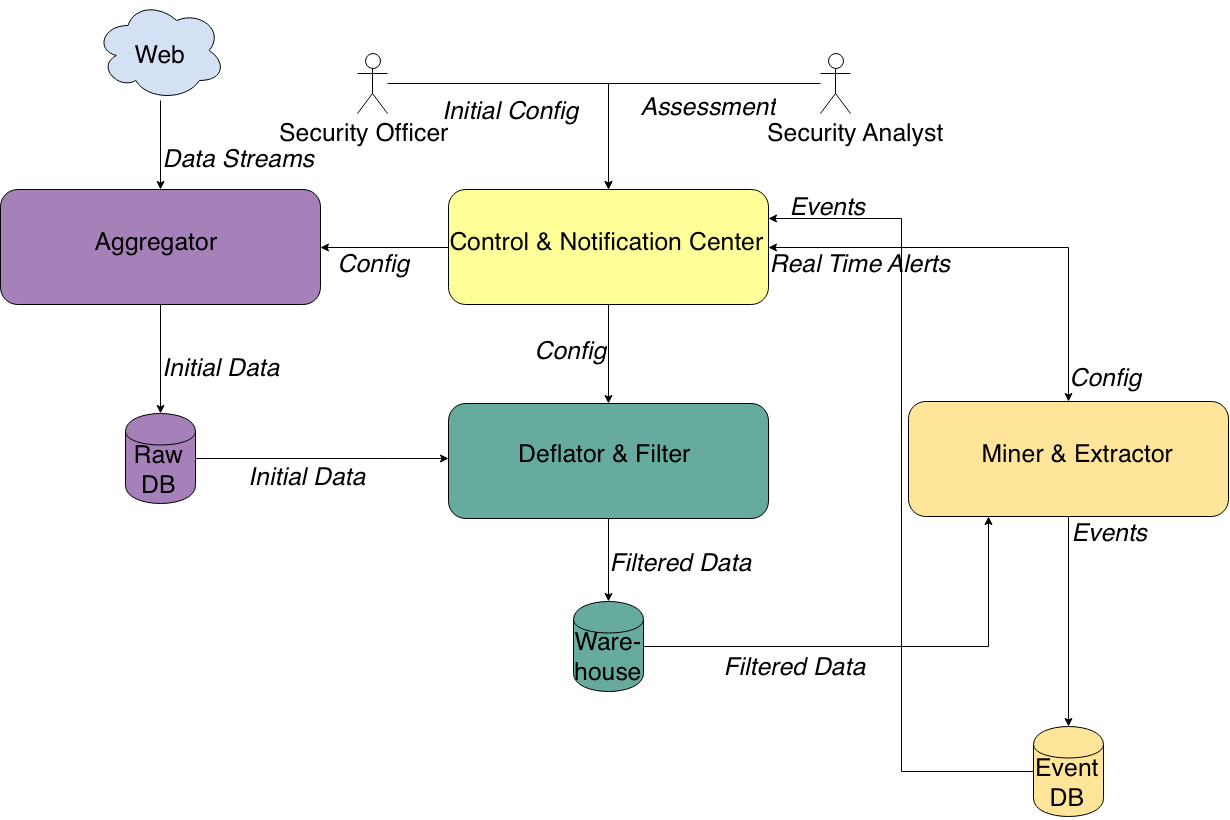
\includegraphics[scale=0.33]{./images/Architecture.png}
    \caption{System Architecture overview}
    \label{fig:arch}
\end{figure}	

\newpage
\subsubsection{Configuration}
The system needs to be as versatile as possible. To that aim each separate part of the system must be able to read a set configuration options that will be inserted into the system through a common control portal. These configuration sets can include (but not be limited to) Data Mining criteria, filtering thresholds, execution intervals for the distinct modules, search keywords, etc. 

\subsubsubsection{Specification}


The most crucial configuration set to the operation of the system is the categorisation of the most common security threats, such as DDoS attacks, malware, exploits and vulnerabilities, etc. This involves the definition of a set of search terms (keywords) associated with each class of threats. Each defined keyword must have an importance level attached to it (weight) denoting the contribution of an occurrence of this word to the score of each document. \\

The next step is to define the sources of information. This can be a very cumbersome task that demands expert knowledge and experience, as well as extensive field survey. This study focuses on data originating from public web sources. This can include websites dedicated to one or more security threats as well as social media (Twitter, Facebook, etc.) where general discussions take place. \\

Having mentioned that we can distinguish two separate categories of sources which we will name 'Targeted' and 'General'. Targeted sources are websites that provide real time information about security related issues. These sources usually provide their information in a format that is structured to some extent. Their constant monitoring can be used to raise alerts without much further processing.\\
General sources are much more unpredictable and unstructured. The data collected from such sources have to be further processed in order for the system to distinguish the important from the not important documents as well as to look for previously unknown patterns hidden in the dataset. \\

%% GIVE EXAMPLES OF THE MODEL FROM THE PDF
%% CHECK AGAIN
\paragraph{Keyword definition}
It is fundamental to outline threat types and define the search keywords correctly as they compose the number of results that one will get from a database. Furthermore, commonly keywords should downgrade their importance when longer time measurements are taken since they will appear more often. The third important factor in defining the correct keywords and their weight is the volume of data being processed to filter out false positives and to get a good hit per ratio comparison. For example once we perform an initial security test of a company with the global keywords( e.g. sql injection, ddos attack) for each company we should make an instance of the agent, with company specific keywords, to add value to the monitored data and get the correct results for each company. Therefore, if we add to the aggregator module specific keywords they might give high performance on certain news highlights in a specific moment, but as we want to protect companies over time after clearing them of the most possible attacks such as sql injections to have a continuous monitoring of their system and to add value to our monitoring we should make a second monitoring instance that is more probed to their specific company needs. To construct and select the relevant keywords, previously discussed news \cite{list-2015-attacks} and messages related to specific threat can be analysed. 

Assuming that our target are all possible general attacks we can select the most common and popular \cite{owasp} and if we associate a list of keywords to some of this threats and apply a search method with the defined list, for a short period of time this can give some good results, once we stretch the time period we will get thousand of hits and this would be a bad selection of keywords.\\


\begin{center} 
\begin{longtable}{|l | l|}
\hline
Type of Attack & Related keywords \\
\hline
 Denial-of-Service (DoS) & ddos attack \\ 
 						& take down website \\ 
 						&  server/computer crush  \\
 						& server take down \\

\hline
SQL Injection 	& plain text password\\
				& clear text password \\
				& plain text password username \\
				& clear text password username\\
				& dump customers \\
				& dump passwords \\
				& blackmail dump accounts \\
				& leaked passwords \\
				
\hline
Account hijacking & account hacked \\
				  & account images changed hack \\
				  & take control account \\
				  & account add/remove content \\ 			  
\hline

\end{longtable}
\end{center}
\paragraph{Source Definition}
\hfill \break \\
Discovering real time threats within an accepable margin of error, is a challenging task. One of the reasons is that the Web is essentially an enormous database filled with random information. Within this chaoitic data space, big amounts of security related knowledge can be discovered. Therefore, it is vital to be able to define the reliable sources that can provide valuable information that will allow us to build Security Intelligence. \\

The question might arise, which sources can be considered as reliable? In order to answer this question expert knowledge has to be gathered. At this point we were provided with a list of possible sources compiled by the developers of the CTI portal in Deloitte. Among all the possible raw data sources, four were recommended to collect a certain amount of data to be used as a testbed.These are Phishtank, Pastebin, Twitter and Reddit. The impotance level of the above websites can be seen via the fact that critical vulnerabilities were revealed through posted messages\cite{list-2015-attacks}.\\
Since this project is focused on the public Web, other sources such as RSS feeds or IRC channels will not be investigated due to time limitations.   

\subsubsubsection{Implementation}
There has been no implementation effort from our side on this particular system module. However, as it has been mentioned before, there is ongoing effort inside the company towards the development of a CTI portal which will be in essence a configuration provider for the rest of the system. This project proposes the integration of the suggested system with the afformentioned CTI portal that will act as the configuration module. 


\subsubsection{Data Aggregation}
After the desired configuration options have been submitted, the  system can start its operation by collecing raw data from the various speficied sources. Since we are dealing with more or less unstructured data, some first form of structure must be given during this step.


\subsubsubsection{Specification}

\subsubsubsection{Implementation}


\paragraph{Twitter}
\hfill \break
Twitter exposes both Streaming and RESTful APIs. While the RESTful approach requires separate HTTP connections for each request to the API, Streaming requires keeping a persistent HTTP connection open \cite{twitteroverview}.\\

For our example we selected the Streaming API approach which provides developers with low latency access to Twitter’s global stream of Tweet data \cite{twitteroverview}.\\

Connecting to the Streaming API requires to provide with authentication details via an OAuth signature. To generate this signature the user has to register their application and generate four parameters named Consumer key, Consumer secret, Access Token and Access token secret.\\

One particular endpoint, provided by the Public Stream \cite{twitterpublic}, was used, namely "POST statuses / filter". This endpoint can be reached via the following URL:\url{https://stream.twitter.com/1.1/statuses/filter.json}.\\

Status filtering allows the user to retrieve tweets that contain certain keywords (up to 400 keywords can be specified), follow specific Twitter users (up to 5000 different users) or retrieve tweets originating from a specific location \cite{twitterfilter}.\\

In our demonstration we only used the keyword (track) option in order to track specific tweets containing security related words (e.g. attack, hack, vulnerability, etc.)\\

The data returned from this particular API call are JSON fomated.\\

The Twitter aggregation agent was developed with the use of Tweepy \cite{tweepy}, an external Python library that provided OAuth authentication and connection to the streaming API.\\ This agent reads its configuration from an external YAML file. This includes Authentication credentials, as well as the specific keywords that we want to track.\\

The sofware parses the returned JSON object, scrapes all unnecessary information (user profile pictures, background colors, etc.) and stores the rest of the information in the database.  

\newpage
\paragraph*{Pastebin}
\addcontentsline{toc}{paragraph}{Pastebin}
\hfill \break
\\
\textit{Pastebin} websites \cite{fpaste} \cite{pastebin} allow everyone with or without registration to share blocks of text or code snippets. They have attracted many users during past years including cybercriminals such as malware developers\cite{pastebin-magazine}. The enormous flow of information ranges from database dumps, containing e-mails and passwords, to harmful backdoor programs. With a deeper examination of these publicly pasted messages possible future attacks may be discovered.\\
\hfill \break
From all possible \textit{pastebins} (e.g. fpaste.org \cite{fpaste}, paste2.org, pastie.org\cite{pastebin-pastie}, 
paste.ubuntu.org.cn \cite{pastebin-ubuntu} etc.) pastebin.com \cite{pastebin} has been selected to be further inspected.
\hfill \break
\\
Pastebin exposes an API that offers different options for developers. More specifically these include creating new pastes, listing trending pastes or the posts of a particular user. The above functionallities can be used once one obtains a unique Developer API Key. 
\hfill \break
\\
At this moment Pastebin API \cite{pastebin} does not offer any option for listing all new messages posted by unregistered users. The only option available, is to list the posts of a specific registered user. However, any information posted might be of potential interest. 
This makes our work rather challenging but not impossible.  
\hfill \break
\\
One could possibly use the search method provided by \textit{Pastebin.com} for retrieving posts containing a combination of keywords.
This functionality, however, makes use of \textit{Google Custom Search}. Therefore, if one desires to retrieve all posts related to certain specified keywords, they would have to use the Google custom search API. This, however, limits free users to 1000 searches per day. 
\hfill \break
\\
To overcome the above limitations and collect all new pastes that arrive, a web crawler module was implemented. \textit{Scrapy} \cite{scrapy}, an open source framework for building extensible webcrawlers was used, integrated into a Python script. Pastebin's \texttt{Archive} page contains all pastes posted during the last 10 minutes. For that reason, we will crawl and fetch the contents of this page each 10 minutes. Not all data from the page provides interest this is why we will scrape the html and keep only the information that is relevant for further examination. This includes the url, the paste, the posting date and the number of unique views. By inspecting the elements required from the DOM tree, we then can parse these nodes and extract only the raw paste text. Once all this data has been gathered, it will be stored in the database.
\paragraph*{Phishtank}
\hfill \break
Phishtank is the only 'targeted' source that we examined in this project. It is a website dedicated to tracking Phishing attempts. Any registered user can submit websites that they suspect of Phishing. Other users can log in later and verify if the website is indeed Phishing or not. Phishtank also informs the user if the website is still online or not.\\

Developing over the Phishtank API is pretty simple and straight forward. Phishtank offers its whole database to be downloaded either in CSV, JSON, XML or serialized PHP format. The database includes all websites that are verified as phishing and are still online, and it is updated every hour. The user is adviced to register their applications and obtain an access token in order not to be constricted by download limits. \\

The aggregator code simply downloads the whole database from the following url \url{http://data.phishtank.com/data/online-valid.json}, parses the json entries and stores in the database all useful information. \\

Since Phishtank is a targeted source, all returned information can be handled directly from the system in order to raise security alerts without much further processing. 
 
\paragraph{Reddit}
\hfill \break
\\
The Reddit community comprises of social media and news sites. It contains over 5000 channels called "subreddits" which belong to different categories. In this project we will collect Reddit \cite{reddit} data originating from the following subreddits:
\begin{itemize}
\item /r/blackhat \cite{r.blackhat}
\item /r/malware \cite{r.malware}
\item /r/netsec \cite{r.netsec}
\item /r/pwned \cite{r.pwned}
\item /r/vrd/ \cite{r.rvd}

\end{itemize}
\hfill \break
\\
Although the Reddit API \cite{reddit} provides a rich list of methods, we have chosen a few of them for the purposes of this project.\\
\hfill \break
In order for a user to list new, top, controversial, etc. messages they would just have to add "/" and the name of the operation they want to perform to the end of the subreddit url in question. The user can provide additional parameters in order to filter, sort, and limit the number of posts retrieved. 
\hfill \break
\\
All ingredients needed for implementing an aggregation agent for Reddit are supplied by the API. The only part we need to add is some filtering capabilities that will allow us to keep the parts of the information that can help with defining the relevance of each document.
\hfill \break
\\
First a connection needs to be opened to the the targeted subreddit, for example /r/blackhat. This is what the following line of code does:

\begin{spverbatim}
response = urllib2.urlopen('http://www.reddit.com/r/blackhat/new
			.json?sort=new&limit=100')
\end{spverbatim}
\hfill \break
\\
The response will be a JSON formated string. From all the fields in the structure we will only store the title, the number of comments and score. It is important to also store the date of each retrieved message, in order to monitor its voting trends within a specific time period.
\hfill \break
\\
All the collected data are stored in the database. 


\subsubsection{Preprocessing \& Filtering}
The documents collected from all the public sources must be given a common format suitable for further analysis. Also the system must be able to easily distinguish which documents carry importance for further Security Analysis. To that aim we propose a 'deflation' and scoring model 


\subsubsubsection{Specification}
\subsubsubsection{Implementation}
\subsubsubsection{Alternative Approaches}
Besides the previously mentioned deflation method we have also tested different options. This subsection will outline some alternative methods for cleaning documents by employing NLP techniques as well as the use of the TF-IDF alghorithm for determining the relevance and importance of each document.
\paragraph{Natural Language Processing}
NLTK or Natural Language Toolkit ...

%removing stop words, stemming and recognizing part of speech with a further

\paragraph{TF-IFD}
\hfill \break
\\
TF-IDF \cite{tf-idf} stands for \textit{Term Frequency–Inverse Document Frequency} and it is used to statistically score the importance of a word in a document or across a collection of documents. A word will be considered important if it appears multiple times into a document. TF is calculated by counting how many times the specific word appears, over the total number of words within that document. If that word appears in other documents as well it will be less unique and thus receive a lower score. That score refers to the IDF calculation. 
\hfill \break 
\\
To determine the documents most relevant to specific keywords, it is first required to define certain query terms relevant to known threat categories. The the algorithm will take the query into account and will produce a statistical list of the most significant documents as a result. This is an automated method for sorting document importance according to a specified search term. 
\newpage
\subsubsection{Analytics and Mining}
This section will sketch few methods that can be applied over the congregated information. All the unstructured data has to be processed and converted to "clean" structured information which includes natural language processing. For this step Python provides an open source library nltk \cite{nltk}. We have to dip into several phases to get a good transformation of  paste, mesages or titles. This includes stop words removal, stemming and pos(part of speach) detection. 
At this moment there are various data mining techniques \cite{oracle-list} that include text processing. Investigating all this techniques is out of scope in this project, therefore the once that are mostly commonly used will be provided. In data mining step or Knowledge Discovery in Databases (KDD) it is important to find and extract patterns and knowledge from database not the data itself \cite{data-kdd}.
\subsubsubsection{Specification}
\subsubsubsection{Implementation}
\subsubsection{Feedback and Assessment}
\subsubsubsection{Specification}
\paragraph{Data mining tasks}
\begin{itemize}
\item 
\textbf{Classification}: Refers to the task of generalising known structures and applying them to new
data. For example, an e-mail program might attempt to classify an e-mail as "legitimate" or as
“spam”. Since this involves training of the algorithm before use, it might not be ideal for use in
threat discovery. However, it can be very useful for providing feedback to the system and fine
tuning it to be able to classify the documents for each threat category, acting together with the
configuration step
\item 
Anomaly detection (Outlier/change/deviation detection): This task refers to identification of
unusual data records that might imply unusual behaviour in the dataset. For example, in our
use case, a first indication that something might be possibly wrong would be an exceptional
mention of a company name within a certain period of time. The problem here is to determine
what can be defined as exceptional. This of course is not possible without the use of old data
so a certain threshold can be determined. Until sufficient amount of data has been gathered we
can naively implement this by setting the thresholds manually. This operation is particularly
popular in intrusion detection systems.
\item 
Association rule learning (Dependency modelling): This task refers to the search for
relationships between variables. One example of this is the infamous beer and diapers story.
This test requires no training set and can be performed on any structured set of data. In our
use case this can help us determine trends between the occurrences of keywords, such as the
name of a company together with the name of a name of an attack. The output of this test also
contains metrics about the support (percentage of the documents supporting the association) as well as
confidence (ratio of the support percentage of either part of each rule).
\item 
Clustering: Refers to the task of discovering groups and structures in the data that present
some sort of similarity, without using known structures in the data. In our case this can help us
determine new categories of documents that have not been predefined (remember the threat
categorisation we mentioned in the beginning).
\item
Regression: This task attempts to find a function which models the data with the least error.
This might not be directly applicable to our specific example but based on the experience
gathered after a certain period of time that the system will be operated, we can attempt to
design an analytic model using regression analysis techniques.
\item
Summarisation: This task aims to provide a more compact representation of the data set,
including visualisation and report generation. In our case this applies to the creation of the
alerts to be presented to the Security Analysts. The alerting will consist of a common format
that will apply to automatically generated events that will be propagated to the appropriate
parties. One proposed format could be the following:
%\{alert\_id: 00001, subject: "Something is rotten in the state of Denmark", importance: Red, backing_documents:\[1,3,4,6\]\}
This presents the analyst with an event informing them about a security incident with a certain importance level. The way of determining the level of importance falls out of the scope of thisn document. Notice also the list of supporting documents resulting from different sources. At this point the analyst can go and inspect each one of this documents manually, assess the risk themselves and take the appropriate measures such as further informing the involved parties, or ignoring the alert.
\end{itemize}
\subsubsubsection{Implementation}
\paragraph*{Association Rule}
\addcontentsline{toc}{paragraph}{Association Rule}
\paragraph*{Clustering}
\addcontentsline{toc}{paragraph}{Clustering}
\hfill \break 
\\
For our specific use case clustering is important for automating the process of finding new type of Secuity threats that occur in a specific period of time. The proposed method groups related documents that belong to a certain cluster (meaning they refer to a spefic topic) and provides a list of the most frequent terms appearing in the cluster.
\\
\\
For clustering N collected documents from the database in K categories an option would be using K-means\cite{k-means} algorithm, also known as Lloyd's algorithm. The method\cite{k-means-example} proposed by this algorithm aims to find K non-overlapping clusters and it works as follows. User specifies how many K clusters will represent the initial centroids, chosen randomly, in which the information will be divided into. Assign each observation point(word) to the closest centroid, where each collection of points(words) form a cluster. The centroid is then updated depending of the words added to this cluster. The process stops when the words assigned will not change the clusters. At this moment there is no guarantee that the result retrieved is optimum. The outcome might be different each time, depending on how the initial centroids are chosen. Important factor to mention here is the selection of K, because an incorrect choice might lead to non-optimum results. There are several procedures\cite{procedures-for-kmeans} to calculate a favourable number of clusters but this is out of scope and the investigation, and we will consider random cluster number that will be feasible chosen compared to the amount of data.
\\
\\
In order to implement the proposed algorithm an open  source scikit- learn \cite{sklearn} tool was used for data analysing that provides a library called SKlearn which can be integrated in Python environment. Following an example provided in a tutorial from the sklearn website, which attemps to categorize 20 news group\cite{k-means-20news}, we adapted it to use the data provided in the database and show what are the documents that are related to each other in a cluster.  In this case we applied the algorithm on over 600000 twitter messages and the expected outcome was to categories this messages in 20 groups. From the clusters obtained two showed big interest as it presents real events that happened in the past weeks.
\begin{spverbatim}
Cluster 13:  paris  charlie  hebdo  attack  http  mayor  nypd  
rt  victims  french  honor  visited  nyc  france  terror  muslim 
 bolsters  security  jewish  cover
Cluster 15:  photos  leaked  upton  kate  jennifer  lawrence 
 nude  victoria  justice  megan  fox  http  seen  rt  hoeuu2dubr  
itweetlikegirls  hilarious  kardashian  kim  aigbtbpmvv
\end{spverbatim}
\hfill \break
Observing the resulted clusters we can claim that the algorithm behaved well considering that it is an unsupervised method and the top frequent terms for Cluster 13, highlights the most recent attack in Paris. In the Cluster 15 which is totally unrelated to the previously mentioned attack, the incident with leaked celebrities photos is outlined.
\paragraph*{Classification}
SVM Algorithm 

\section{Results}
\subsection{Demo}
\newpage
\section{Conclusions}



\newpage
\section{Future Work}

At this moment we have implemented a modular and pipelined system by using open source tools. As a future extension, one target would be to have a full system implementation. This system can be further integrated with already developed CTI (Cyber Threat Intelligence) portal. Due to the lack of time, we have build a simple training set in the classification module, just to showcase that it is a feasible attempt to categorize a new given set of items based on the previous trained set. A normal step would be to build numerous training sets from the real world data, gathered from social websites, and test them on the new incoming data. This step requires time as new attacks might happen in a week, month or year. Therefore at least one year would be necessary to have a stable, favourable trained set. Classification method can also be used for exploring sentiment analyses for the collected messages. To build a set that will distinguish false positives, at first this can be done manually by a Security Analyst which could split a real attack from just a random message. Moreover, natural language processing capabilities can be explored to filter messages from all the unnecessary data and retrieve only the interesting data that can be further structured for a further analyse. Clustering method that we proposed for finding new categories of attacks that might have been omitted, uses a random K number defined by user. For optimised results, a good solution would be to check the proposed methods for finding the optimal number of clusters in a given dataset. An expected outcome for the assessment module would be the ability to rise real time alerts in the moment a threat or attack to certain company or client is found.

\newpage
\section{Appendix}
\newpage

\begin{thebibliography}{99}
\bibitem{cyber}
US cybercrime: Rising risks, reduced readiness, PWC, Available at: \url{http://www.pwc.com/en_US/us/increasing-it-effectiveness/publications/assets/2014-us-state-of-cybercrime.pdf}
\bibitem{sony}
	 D. Sanger, N. Perlroth.  U.S. Said to Find North Korea Ordered Cyberattack on Sony. [online] Nytimes.com. \\Available at: \url{http://www.nytimes.com/2014/12/18/world/asia/us-links-north-korea-to-sony-hacking.html?_r=0}
\bibitem{socialweb}
  Russell, MA (2014). Mining the Social Web, O'Reily Media, USA
\bibitem{minds}
    V. Chandola et al. Data Mining for Cyber Security, Department of Computer Science, University of Minnesota, Springer, 2006
\bibitem{police}
   RCP van der Veer, H.T. Roo,  A. van der Zanden, Data mining for intelligence led policing, Sentient, Amsterdam Police Force, Amsterdam, The Netherlands, 2009
\bibitem{nltk}
Nltk.org, (2015). Natural Language Toolkit - NLTK 3.0 documentation. [online] Available at: \url{http://www.nltk.org/}

\bibitem{fpaste}
Fedora Project Pastebin Fpaste.org, (2015). New paste • Fedora Project Pastebin. [online] Available at:  
\url{http://fpaste.org }
\bibitem{pastebin}
Pastebin, (2015). Pastebin.com - \#1 paste tool since 2002!. [online] Available at:     \url{http://pastebin.com/}

\bibitem{pastebin-magazine}
Security Intelligence, (2015). Pastebin a Convenient Way for Cybercriminals to Remotely Host Malware. [online] Available at: \url{http://securityintelligence.com/news/pastebin-convenient-way-cybercriminals-remotely-host-malware/#.VMS25DX8vCI }
\bibitem{pastebin-pastie}
Pastie.org, (2015). New - Pastie. [online] Available at: \url{http://pastie.org} 
\bibitem{pastebin-ubuntu}
 Paste.ubuntu.org.cn, (2015). [online] Available at: \url{http://paste.ubuntu.org.cn/}
\bibitem{scrapy}
Scrapy.org, (2015). Scrapy | A Fast and Powerful Scraping and Web Crawling Framework. [online] Available at: \url{http://scrapy.org/} 
\bibitem{reddit}
Reddit.com, (2015). reddit: the front page of the internet. [online] Available at: \url{http://www.reddit.com/} 
\bibitem{r.blackhat}
Reddit, (2009). blackhat library: Documenting blackhat hacking techniques • /r/blackhat. [online] Available at: \url{https://www.reddit.com/r/blackhat}
\bibitem{r.malware}
Reddit, (2009). Malware Analysis \& Reports • /r/Malware. [online] Available at:   \url{http://www.reddit.com/r/malware}
\bibitem{r.netsec}
reddit, (2007). /r/netsec - Information Security News \& Discussion. [online] Available at: \url{https://www.reddit.com/r/netsec/} 
\bibitem{r.pwned}
Reddit, (2008). pwned • /r/pwned. [online] Available at: http://www.reddit.com/r/pwned 
\bibitem{r.rvd}
Reddit, (2012). Vulnerability Research and Development • /r/vrd. [online] Available at: \url{http://www.reddit.com/r/vrd/}
\bibitem{oracle-list}
Oracle.com, (2015). Oracle Data Mining Techniques and Algorithms. [online] Available at: \url{http://www.oracle.com/technetwork/database/enterprise-edition/odm-techniques-algorithms-097163.html}
\bibitem{tf-idf}
Tfidf.com, (2015). Tf-idf : A Single-Page Tutorial - Information Retrieval and Text Mining. [online] Available at: \url{http://www.tfidf.com/} 
\bibitem{data-kdd}
Han, Jiawei; Kamber, Micheline (2001). Data mining: concepts and techniques. Morgan Kaufmann. p. 5. ISBN 9781558604896. "Thus, data mining should have been more appropriately named "knowledge mining from data," which is unfortunately somewhat long"
\bibitem{owasp}
Owasp.org, (2015). Category:OWASP Top Ten Project - OWASP. [online] Available at: \url{https://www.owasp.org/index.php/Top10#OWASP_Top_10_for_2013} 
\bibitem{list-2015-attacks}
Passeri, P., Passeri, P. and Passeri, P. (2015). Cyber Attacks Timeline | Hackmageddon.com. [online] Hackmageddon.com. Available at: http://hackmageddon.com/category/security/cyber-attacks-timeline/ 
\bibitem{sklearn}
Scikit-learn.org, (2015). scikit-learn: machine learning in Python — scikit-learn 0.15.2 documentation. [online] Available at: \url{http://scikit-learn.org/stable/index.html}
\bibitem{orange}
Bioinformatics Laboratory, U. (2015). Orange Data Mining. [online] Orange.biolab.si. Available at: \url{http://orange.biolab.si/} 
\bibitem{k-means} Junjie Wu , Advances in K-means Clustering: A Data Mining Thinking
\bibitem{k-means-example}
Gonçalves, H. (2015). K-means clustering - algorithm and examples. [online] Onmyphd.com. Available at: \url{http://www.onmyphd.com/?p=k-means.clustering}
\bibitem{procedures-for-kmeans}    Glenn W. Milligan, Martha C. Cooper , An examination of procedures for determining the number of clusters in a data set
\bibitem{k-means-20news}
Scikit-learn.org, (2015). Clustering text documents using k-means — scikit-learn 0.15.2 documentation. [online] Available at: \url{http://scikit-learn.org/stable/auto_examples/document_clustering.html} 
 
\end{thebibliography}
\end{document}
